\documentclass[a4paper, dvipdfmx]{article}

%% Language and font encodings
\usepackage[english]{babel}
\usepackage[utf8x]{inputenc}
\usepackage[T1]{fontenc}

%% Sets page size and margins
\usepackage[a4paper,top=3cm,bottom=2cm,left=3cm,right=3cm,marginparwidth=1.75cm]{geometry}

%% Useful packages
\usepackage{amsmath}
\usepackage{graphicx}
\usepackage[colorinlistoftodos]{todonotes}
\usepackage[colorlinks=true, allcolors=blue]{hyperref}
\usepackage{braket, comment, float, tabularx, booktabs} % newly added by Kensuke

\title{A Survey for the Methodology of the Theories on Cumulative Cultural Evolution}
\author{Kensuke ITO\footnote{Ph.D. student., Graduate School of Interdisciplinary Information Studies., The University of Tokyo.}}
\date{}

\begin{document}
\maketitle

\begin{abstract}
    Why only human-beings acquired complex cultural traits? In this research, we survey the theories on cumulative cultural evolution that has been dealing with this question. This is important because cultural evolution is so interdisciplinary a research field as not able to sufficiently systematize existing methods even though we focused only on cumulative and theoretical aspects.

    In order for terse classification, preceding researches were arranged according to two criteria chronological and methodological. As a result, the former depicted, as already pointed out by Horiuchi (2012), that the current theoretical approach is largely based on learning hypothesis and population hypothesis. On the other hand, the latter suggested the circumstances where methods are still miscellaneous and arbitrarily set to obtain predetermined conclusions.

    Therefore, this survey concludes it is necessary for agents' learning and inheritance process to have the consistent assumptions supported by empirical studies. While there are potential constraints, working on this issue with reference to other disciplines would strongly contribute to the further development of theoretical research on cumulative cultural evolution.

    \begin{center}
        Keywords: {\it cumulative cultural evolution, survey paper, theoretical models}
    \end{center}
\end{abstract}

\section{Introduction}

In current studies on cultural evolution, included {\it cumulative} aspects are dealt with more explicit than ever through several discussions we describe later. They are distinguished as {\it cumulative cultural evolution} having the following definitions and research questions for example:

\subsubsection*{Definitions}
\begin{quotation}
    “{\it Human cumulative culture combines high-fidelity transmission of cultural knowledge with beneficial modifications to generate a 'ratcheting' in technological complexity, leading to the development of traits far more complex than one individual could invent alone}”. Dean et al. (2014)
\end{quotation}
\begin{quotation}
    “{\it the preservation of cultural traits over successive generations such that individuals acquire knowledge that exceeds what any single individual could invent alone}”. Mesoudi (2016)\footnote{He also defined culture itself in Mesoudi (2011a) as follows, “{\it culture is information that is acquired from other individuals via social transmission mechanisms such as imitation, teaching, or language}”.}
\end{quotation}

\subsubsection*{Research Questions}

\begin{itemize}
    \item Why only human-beings appear to have complex cultural traits?
    \item What factors will affect the cumulative speed of cultural traits?
\end{itemize}
Contrary to the relatively clear concepts above, however, related researches are still so interdisciplinary\footnote{As far as I covered, they cross anthropology, biology, psychology, sociology and even economics.} as not able to sufficiently systematize existing methods even though we focused only on theoretical fields. Hence, this paper surveys theories of cumulative cultural evolution for better comprehension of the field. In order for terse classification, it is composed of three main sections. First, we review preceding studies in chronological order to clarify how current arguments have been developed. Then, we review them again according to modeling methods especially for learning and inheritance behavior of agents in order to confirm more detailed designs. Finally, implications derived from these two are explained as conclusion.

\section{Chronological Review}

In this section, preceding researches are reviewed by chronological order. Specifically, their relationships are depicted in Figure 1 and will be explained by dividing into three periods for intuitive understanding: in 1980's, from the late 1990's to the early 2000's and from the late 2000's to 2010's.

\begin{figure}[H]
  \centering
  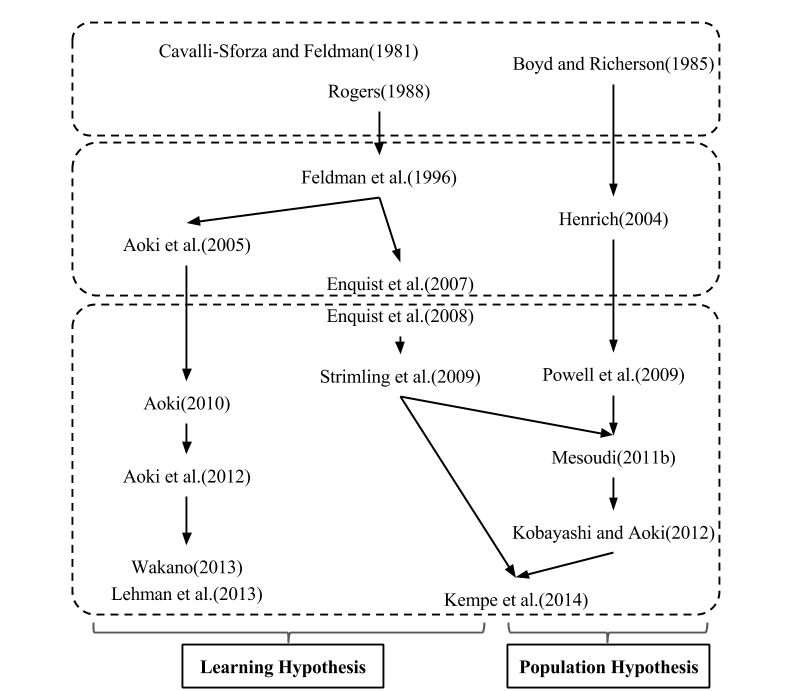
\includegraphics[width=12cm]{fig2_1.png}
  \caption{Relationships of representative theoretical researches on cumulative cultural evolution}
  \label{Figure1}
\end{figure}

\subsection*{Cultural evolution as an research field in the 1980's}
The idea to comprehend culture by an analogy with biological evolution have existed for a long time in anthropology represented by Tylor (1891). However, it was in the 1980's that cultural evolution came to be explicitly treated as one research field. Theoretical researches at the time have a great academic significance in that they extended the model to appropriate forms considering differences from culture, while being based on population genetics. Furthermore, despite the fact that there was no concept of cumulative cultural evolution yet, several important notions have already been presented. Cavalli-Sforza and Feldman (1981), for example, proposed {\it biased-transmission} which means the possibility for agents to imitate culture from other than genetic parents, and Boyd and Richerson (1985) proposed {\it guided variation} denoting that agents can intentionally change acquired cultural traits. They are closely related to social learning and individual learning described in the next section, respectively. In addition, what is especially important during this period is an argument left by Rogers (1988) that the entire fitness of population to environment would not improve even if social learning as a new option were added to individual learning. This problem is later called as Rogers's paradox and induces several studies leading to cumulative cultural evolution.

\subsection*{Researches on cumulative aspects from the late 1990's to the early 2000's}
After the period of stagnation for a while, two main movements began to focus on the cumulative aspect of culture. One is the reply to Rogers's paradox by Aoki et al. (2005) and Enquist et al. (2007). By applying Feldman (1996) model, they revealed that social learning, which had been considered ineffective in Rogers (1988), is actually effective when assuming the accumulation of culture. The other is to consider the influence of population by Henrich(2004). His model, referring stochastic method by Boyd and Richerson (1985) and the case in Tasmanian islands, revealed that the number of population has a positive contribution to cultural accumulation. These are the beginnings of research on cumulative cultural evolution.

\subsection*{Development and segmentation from the late 2000's to 2010's}
Since the late 2000's, cumulative cultural evolution research came to the era of development accompanied by segmentation. Aoki et al. (2005) and Enquist et al. (2007) who worked on Rogers's paradox with a similar approach have also gradually been separating their research themes. The former developed into researches on learning strategies dealing with the problems such as in what order do agents perform social and individual learning in their lifetime, and what is the optimal allocation of their resources (Aoki (2010), Aoki et al. (2012), Wakano (2013), Lehman et al. (2013)). The latter, then, developed into studies focusing on the accumulation of the resulting cultural traits themselves rather than agents' strategy (Enquist et al. (2008), Strimling et al. (2009)). Particularly, Strimling et al. (2009) proposed interesting implication that, while social learning accuracy and innovation rate can contribute to cultural accumulation, population is not necessarily important in a given condition. On the other hand, researches for population also continued to develop by extending Henrich (2004). For example, Mesoudi (2011b) analyzed the influence on acquisition cost of cultural traits; and subsequently, Kobayashi and Aoki (2012) did more elaborate research for population effect by more realistic model which contains overlapping generation and constraint on the number of candidates of cultural parents.

Current theoretical researches having the above circumstances, as pointed out by Horiuchi (2012), can be classified as {\it learning hypothesis} and {\it population hypothesis} according to their roots. That is, researches rooted for Rogers's paradox are attributing the solution of aforementioned research questions to learning pattern, whereas researches based on Henrich (2004) are population. What is important here is that both hypotheses are complementary and compatible, and theoretical models in each side are not conflicting relationships. In fact, the boundary between the two hypotheses has become more ambiguous among recent researches. In Kempe et al. (2014), for example, both social learning fidelity and multiple demonstrators are implied to be effective; each corresponds to learning and population, respectively.

\subsection*{Summary}
We have thus far seen the brief history of the theories up to the formation of contemporary arguments. Cultural evolution as an research field appeared in 1980's by extending Darwinian evolutionary theory to cultural phenomena. Then, theories of cumulative cultural evolution had been developed by two backgrounds: an answer of Rogers's paradox and an expression of population effects. Nowadays, studies have been gradually segmented inside the two complemental hypotheses: Learning hypothesis and Population hypothesis. Although such whole relationship is clear and consistent, for the more detailed survey it is also necessary to confirm the structure of each model. In the next section, therefore, adopted modeling methods in representative models will be investigated.


\section{Methodological Review}

This section classifies aforementioned representative theories with respect to adopted methods. This is by no means easy because of the large structural difference for each theoretical model. Thus, in this survey, we will simplify the process of cultural accumulation to the generalized framework shown in Figure 2 and discuss its three main components: social learning, individual learning and inheritance.

\begin{figure}[H]
  \centering
  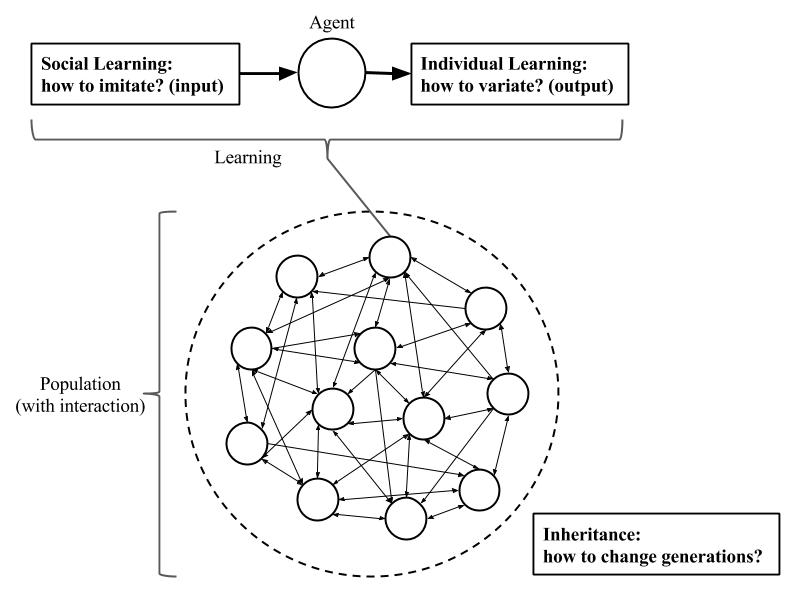
\includegraphics[width=12cm]{fig2_2.png}
  \caption{A simplified framework for theories on cumulative cultural evolution}
  \label{Figure2}
\end{figure}

\subsection*{Social Learning}
Social learning, which has the following definitions by Boyd and Richerson (1985), is considered to be a particularly important element in cumulative cultural evolution because of the historical background about Rogers's paradox mentioned in the previous section.

\begin{quotation}
    “{\it the nongenetic transfer of patterns of skill, thought, and feeling from individual to individual in a population or society}”. Boyd and Richerson (1985), p34.
\end{quotation}
\begin{quotation}
    “{\it the transmission of stable behavioral dispositions by teaching or imitation}”. Boyd and Richerson (1985), p40.
\end{quotation}

\noindent In terms of modeling, we need to investigate two points in which adopted method would vary, selection of cultural parents and fidelity of transmission. Intuitively, the former is an argument on “who will agents learn cultural traits from ?” and has a long history since its framework was first proposed by Cavalli-Sforza and Feldman (1981) and Boyd and Richerson (1985). There, paths of cultural transmission are classified into three patterns: from their genetic parents (vertical), from the agents of same generation (horizontal) and from parental generation with no genetic relations (oblique). In addition, cultural evolutionists applied psychological bias for the criteria to choose particular cultural parents that is required except for the case of vertical transmission. These classifications and explanations are summarized in Table 1 below. In Henrich (2004) categorized as content bias, for example, agents imitate cultural traits with the highest fitness in population. Agents in Lehman et al. (2013) can acquire information from cultural traits possessed by both an average parental agents (oblique) and other agents existing at the same time (horizontal) depending on their growth period. It is also popular to simplify the choosing process to be stochastic especially for the models not dealing with learning strategies.

\begin{table*}[hbt]
    \centering
    \caption{Modeling methods for selecting cultural parents in social learning}
    \begin{tabularx}{.9\linewidth}{XXX}
        \toprule
        Methods for SL & Biases & Researches \\
        \midrule
        {\it Vertical transmission}: Agents imitate cultural traits only from their genetic parents. & - & Aoki et al. (2012), Wakano (2013) \\ \midrule
        {\it Horizontal or Oblique transmission}: Agents can imitate cultural traits from both agents of same generation (horizontal) and parental generation with no genetic relation (oblique). & {\it Content bias (direct bias)}: Agents imitate cultural traits with the highest fitness in population. & Henrich(2004) \\ \cmidrule{2-3}
                & {\it Conformist bias (Frequency-dependent bias)}: Agents imitate the most popular cultural traits in population. & Lehman et al. (2013)\footnote{Note that, strictly speaking, it is different from content bias since infant agents in Lehman et al. (2013) acquire not the majority, but the average cultural traits of parental generation.} \\ \cmidrule{2-3}
                & {\it Stochastic}: Agents randomly imitate cultural traits in population. & Strimling et al. (2009), Kobayashi and Aoki (2012), Kempe et al. (2014) \\
                \bottomrule
    \end{tabularx}
\end{table*}

The latter, fidelity of transmission should also be noted. In several theories represented by Strimling et al. (2009), social learning would not always be succeed even if cultural parents were selected by agents. This is because their models assume social learning efficiency as an exogenous variable in order to analyze imperfect transmission that can occur in reality.


\subsection*{Individual Learning}
Individual learning, on the other hand, has the following definition by Mesoudi (2011b) for example.

\begin{quotation}
    “{\it the process of learning on our own with no influence from other individuals}”. Mesoudi (2011b), p4.
\end{quotation}

\noindent In other words, it means the notion of cultural variation, which could induce cultural accumulation by combining with social learning. Main methods for individual learning are shown in Table 2. One of the simplest modeling ways is stochastic variation represented by Henrich (2004). In his model, agents are assumed to variate acquired cultural traits according to Gumbel distribution. Accordingly, as the population increases, cultural traits with high fitness are stochastically more likely to appear and they are imitated and inherited by social learning with content bias. Thus, positive effect of the number of population on cumulative culture can be concisely expressed.

Especially in studies on learning strategies, on the other hand, individual learning is often modeled by a function type requiring resources such as labor and time. It is linear in most cases, and as shown in guided variation of Boyd and Richerson (1985), the purpose of the model is to maximize the fitness of cultural traits. Although calculations of learning ESS (evolutionary stable strategy) by Aoki et al. (2012), Wakano (2013) and Lehman et al. (2013) are all based on the fitness of not cultural traits but agents, both fitnesses are associated with each other on the assumption that agents can increase their own fitness by obtaining a lot of cultural traits or mutating them suitable for the environment.

Another popular method, called intermediate here, is to put exogenous parameter for individual learning to the model. In Strimling et al. (2009) model, for example, the expected number of new cultural traits produced by an agent is expressed as innovation rate. One of the biggest differences from functional type variation is that there is no resources as input and parameters are sometimes treated as random numbers to analyze heterogeneous agents.

\begin{table*}[hbt]
    \centering
    \caption{Modeling methods for individual learning and related researches}
    \begin{tabularx}{.9\linewidth}{XXX}
        \toprule
        Methods for IL & Researches \\
        \midrule
        {\it Stochastic}: Cultural variation follows a given probability distribution. & Henrich (2004) \\ \midrule
        {\it Intermediate}: Cultural variation follows exogenous parameter which can be determined randomly. & Enquist et al. (2008), Strimling et al. (2009), Kempe et al. (2014) \\ \midrule
        {\it Functional}: Cultural variation follows a given function type. (mostly linear) & Guided variation in Boyd and Richerson (1985), Aoki et al. (2012), Wakano (2013), Lehman et al. (2013) \\ \bottomrule
    \end{tabularx}
\end{table*}

\subsection*{Inheritance}
The methods for Inheritance can be classified into two types as shown in Table 3, discrete and overlapping. The former denotes the structure where parental agents produce offspring agents, accompanied by genetic or cultural inheritance. Discrete methods tend to be adopted by the studies on learning strategies which focus on individual properties rather than populations and are often assumed that offsprings imitate the cultural traits or learning strategies of parental generation. However, it is important to note that the discrete method does not always mean vertical transmission. For example, Lehman et al. (2013) having a discrete style, introduced horizontal and oblique transmissions which are simplified in preceding models, and offered generalization of Rogers's paradox by the implication that culture can accumulate only in the case of oblique transmission. On the other hand, the latter denotes the structure where entry of new agents and retire of a part of existing agents are repeated within the population. In this case there are almost no restrictions on social learning, and the method for selecting demonstrator varies depending on the model. Overlapping method was originally applied to the individual models like Strimling et al. (2009), but now it is extended to the population models rooted for Henrich (2004).

\begin{table*}[hbt]
    \centering
    \caption{Modeling methods for inheritance and related researches}
    \begin{tabularx}{.9\linewidth}{XX}
        \toprule
        Methods for Inheritance & Researches \\
        \midrule
        {\it Discrete}: Parental agents create offspring agents, accompanied by genetic or cultural inheritance. & Henrich (2004), Aoki et al. (2012), Wakano (2013), Lehman et al. (2013) \\ \midrule
        {\it Overlapping}: Entry of new agents and retire of a part of existing agents are repeated within the population. & Strimling et al. (2009), Kobayashi and Aoki (2012), Kempe et al. (2014) \\ \bottomrule
    \end{tabularx}
\end{table*}

\subsection*{Summary}
This section covered miscellaneous methods in the theories on cumulative cultural evolution. In the modeling of social learning, there were two points in which adopted method varies, cultural parents and transmission fidelity. As for individual learning, various functional forms were proposed according to its purpose and strategy. Methods for inheritance, then, could be divided into discrete and overlapping.

It should also be noted that the implications of the model are completely different depending on the methods placed. As shown in the previous section, current theories are attempting to elucidate the accumulation process of culture from various perspectives such as population, learning strategy and fidelity of social learning; however, contrary to their clear purposes, arbitrariness still remains with regard to method selection. It means, even some assumptions were experimentally supported, the criteria for how to select and combine them would not be consistent and they are fluctuating according to the purpose of the model. Frankly speaking, methods appear to be chosen for deriving pre-determined conclusions.


\section{Conclusion}
In this paper, we have surveyed preceding theories on cumulative cultural evolution from both chronological and methodological views. The former listed its brief but consistent academic history from the early stage when researches for cumulative aspects emerged from the then cultural evolution, to the present stage when main topics were segmented and the persuasive hypotheses were formed. Meanwhile, the latter showed an inconsistent situation that there is still no clear consensus on miscellaneous existing methods and each theoretical model arbitrarily adopts suitable methods for predetermined conclusions.

Therefore, to conclude, this survey asserts the necessity of consistent assumptions to modeling methods on learning and inheritance behavior. In order for taking consistency, assumptions would require further simplification and generalization as already done in other fields represented by economics and multi-agent systems; moreover, much more importantly, they have to obtain sufficient validity supported by empirical or experimental studies and thereby accepted among researchers.

Nevertheless, theoretical and empirical researches are still not in complemental situation for several reasons. One of the most critical reasons would be the technical difficulty of experiment on cultural traits as {\it genotypes}. While researches on biological evolution have greatly developed due to the discovery of genes as fundamental units for information transmission, corresponding units\footnote{They are also called as {\it meme} as an analogy of gene.} have not yet been confirmed in cultural evolution, and most empirical studies alternatively deal with cultural {\it phenotypes} such as arrowheads shape and language variation. However, especially in cumulative cultural evolution, how agents imitate, variate and inherit cultural traits are extremely important issues for research questions, and quantification of culture as {\it genotypes} is inevitable to elucidate their mechanisms. Thus, it will also be worth researching cultural {\it genotypes} for establishing consistent assumptions to modeling methods.

\vspace{20pt}

\begin{flushleft}
\begin{thebibliography}{1}
\makeatletter
\def\@biblabel#1{}
\let\old@bibitem\bibitem
\def\bibitem#1{\old@bibitem{#1}\leavevmode\kern-\bibindent}
\makeatother
\bibitem{ao05} Aoki, K., Wakano, J. Y., Marcus, W. Feldman. (2005), ``The emergence of social learning in a temporally changing environment: a theoretical model'', {\it Current Anthropology}, Vol. 46, No. 2, pp. 334-340
\bibitem{ao11} Aoki, K., Lehman, L., Marcus, W. Feldman. (2011), ``Rates of cultural change and patterns of cultural accumulation in stochastic models of social transmission'', {\it Theoretical Population Biology}, 79, 192–202
\bibitem{ao12} Aoki, K., Wakano, J. Y., Lehmann, L. (2012), ``Evolutionarily stable learning schedules and cumulative culture in discrete generation models'', {\it Theoretical Population Biology}, 81:300-30
\bibitem{bo85} Boyd, R., and Richerson, P. J. (1985), {\it Culture and the evolutionary process}. Chicago, IL: University of Chicago Press.
\bibitem{ca81} Cavalli-Sforza, L. L., and Feldman, M. W. (1981), {\it Cultural transmission and evolution}, Princeton: Princeton University Press.
\bibitem{de14} Dean, L. G., Gill, L. Vale, Kevin., N. Laland., Emma, Flynn., Rachel L. Kendal. (2014), ``Human cumulative culture: a comparative perspective'', {\it Biol. Rev}, 89, pp. 284–301. 284 doi: 10.1111/brv.1205
\bibitem{en07} Enquist, M., Eriksson, K., and Ghirlanda, S. (2007), ``Critical social learning: a solution to Rogers’s paradox of nonadaptive culture'', {\it Am. Anthropol}, 109, 727-734.
\bibitem{en08} Enquist, M., Ghirlanda, S., Jarrick, A., Wachtmeister, C. A. (2008), ``Why does human culture increase exponentially?'', {\it Theoretical Population Biology}, 74 (1), 46–55.
\bibitem{fe96} Feldman, M.W., Aoki, K., Kumm, J. (1996), ``Individual versus social learning: evolutionary analysis in a fluctuating environment'', {\it Anthropol. Sci}, 104, 209-232.
\bibitem{he04} Henrich, J. (2004), ``Demography and cultural evolution: How adaptive cultural processes can produce maladaptive losses The Tasmanian case'', {\it American Antiquity}, 69(2), 197–214.
\bibitem{ke14} Kempe, M., Stephen, J. Lycett., Mesoudi, A. (2014), ``From cultural traditions to cumulative culture: parameterizing the differences between human and nonhuman culture'', {\it Journal of Theoretical Biology}, Volume 359, 21 October 2014, 29–36
\bibitem{enca} Kobayashi, Y., and Aoki, K. (2012), ``Innovativeness, population size and cumulative cultural evolution'', {\it Theoretical Population Biology}, 82 (2012) 38–47
\bibitem{le13} Lehmann, L., Wakano, JY., Aoki, K. (2013), ``On optimal learning schedules and the marginal value of cumulative cultural evolution'', {\it Evolution}, 2013 May;67(5):1435-45. doi: 10.1111/evo.12040. Epub 2013 Jan 23.
\bibitem{me11a} Mesoudi, A. (2011a), {\it Cultural evolution: how darwinian theory can explain human culture and synthesize the social sciences}, Chicago, IL: University of Chicago Press.
\bibitem{me11b} Mesoudi, A. (2011b), ``Variable cultural acquisition costs constrain cumulative cultural evolution'', {\it PLoS ONE 6(3): e18239}, doi:10.1371/journal.- pone.0018239
\bibitem{me11c} Mesoudi, A. (2016), ``Cultural evolution: integrating psychology, evolution and culture'', {\it Current Opinion in Psychology}, 7:17–22.
\bibitem{po09} Powell A, Shennan S, Thomas MG (2009), ``Late pleistocene demography and the appearance of modern human behavior'', {\it Science}, 324: 1298–1301.
\bibitem{ro88} Rogers, A.R. (1988), ``Does biology constrain culture?'' {\it Am. Anthropol}, 90, 819-831.
\bibitem{st09} Strimling, P., Sjostrand, J., Enquist, M., Eriksson, K. (2009), ``Accumulation of independent cultural traits'', {\it Theoretical Population Biology}, 76: 77–83.
\bibitem{ho12} 堀内史朗 (2012), 「資源分配と交流の起源学習」文部科学省科学研究費補助金(新学術領域研究)交替劇B01班2012年度研究報告書
\bibitem{wa13} 若野友一郎 (2013), 「学習と活用のトレードオフ:蓄積的文化進化における最適な学習スケジュール」文部科学省科学研究費補助金(新学術領域研究)交替劇B01班2013年度研究報告書
\end{thebibliography}
\end{flushleft}


\end{document}
